\section{Work-in-progress: \\ private \knn{} queries}

	\begin{frame}{General idea}

		\begin{itemize}
			\item<1->
				Model: \alert{snapshot}, query type: \alert{\knn{}} in arbitrary dimensions

			\item<2->
				Input: vector of real numbers, query: return $k$ ``closest'' inputs to given vector \\
				\begin{small}
					Distance can be $\text{L}_\text{p}$ (usually, Euclidean, $p = 2$) or inner (dot) product
				\end{small}

			\item<3->
				Applications range from similarity search to geographical search \\
				\begin{small}
					Document is a vector of words/features/topics, query is to find $k$ most similar documents \\
					Object on a map is a 2D vector, query is to find $k$ nearest locations
				\end{small}

			\item<4->
				\emph{Approximate distance-comparison preserving encryption (DCPE) scheme} on input and queries
				\[
					\forall x, y, x \in \mathbb{X} : \algo{Dist}{x, y} < \algo{Dist}{x, z} - \beta \implies \algo{Dist}{f(x), f(y)} < \algo{Dist}{f(x), f(z)}
				\]

			\item<5->
				Prove theoretically and observe empirically how accuracy and efficiency of attacks drop with higher security
		\end{itemize}

	\end{frame}

	\begin{frame}{Component: DCPE}

		\[
			\forall x, y, x \in \mathbb{X} : \algo{Dist}{x, y} < \algo{Dist}{x, z} - \beta \implies \algo{Dist}{f(x), f(y)} < \algo{Dist}{f(x), f(z)}
		\]

		\begin{itemize}
			\item<1->
				The scheme is by Riddhi Ghosal and Adam O'Neil
			\item<2->
				\textbf{Key generation}: sample at random length multiplier $s$ and seeds for samplers $K$
			\item<3->
				\textbf{Encrypt}: take input vector $x \in \RR^d$
				\begin{itemize}
					\item Sample nonce $n$
					\item Using nonce and seeds, sample a point $a$ on a $\beta$-radius $d$-dimensional ball
					\item New vector is extended times $s$ and points to $a$
				\end{itemize}
			\item<4->
				\textbf{Decrypt}: take encrypted vector $c \in \RR^d$ and nonce $n$
				\begin{itemize}
					\item Do same steps except \emph{shrink} times $s$ and \emph{remove} ball component
				\end{itemize}
		\end{itemize}

	\end{frame}

	\begin{frame}{Component: TREC dataset and FAISS~\cite{faiss}}

		\begin{itemize}
			\item<1->
				Dataset is 8.8M documents represented as vectors of 768 dimensions \\
				\begin{small}
					Thanks Hamed Zamani for the dataset
				\end{small}

			\item<2->
				Query is a 768-dimensional vector asking for $k = 1000$ closest (inner product) documents

			\item<3->
				% cspell:disable-next-lin
				Original document set is a \textbf{T}ext \textbf{RE}trieval \textbf{C}onference (TREC) test collection \\
				\begin{small}
					set of documents, set of topics (questions), and corresponding set of relevance judgments (right answers)
				\end{small}

			\item<4->
				FAISS~\cite{faiss}: GPU-enabled library for efficient similarity search and clustering of dense vectors
				\begin{small}
					Developed and maintained by Facebook AI
				\end{small}

			\item<5->
				General algorithm: for different $\beta$
				\begin{itemize}
					\item Encrypt dataset with $\beta$
					\item Encrypt queryset with $\beta$
					\item Run queries with FAISS
					\item Generate TREC metrics (using relevance judgments)
				\end{itemize}

		\end{itemize}

	\end{frame}

	\begin{frame}{Intermediate results}

		\begin{figure}[h]
			\centering
			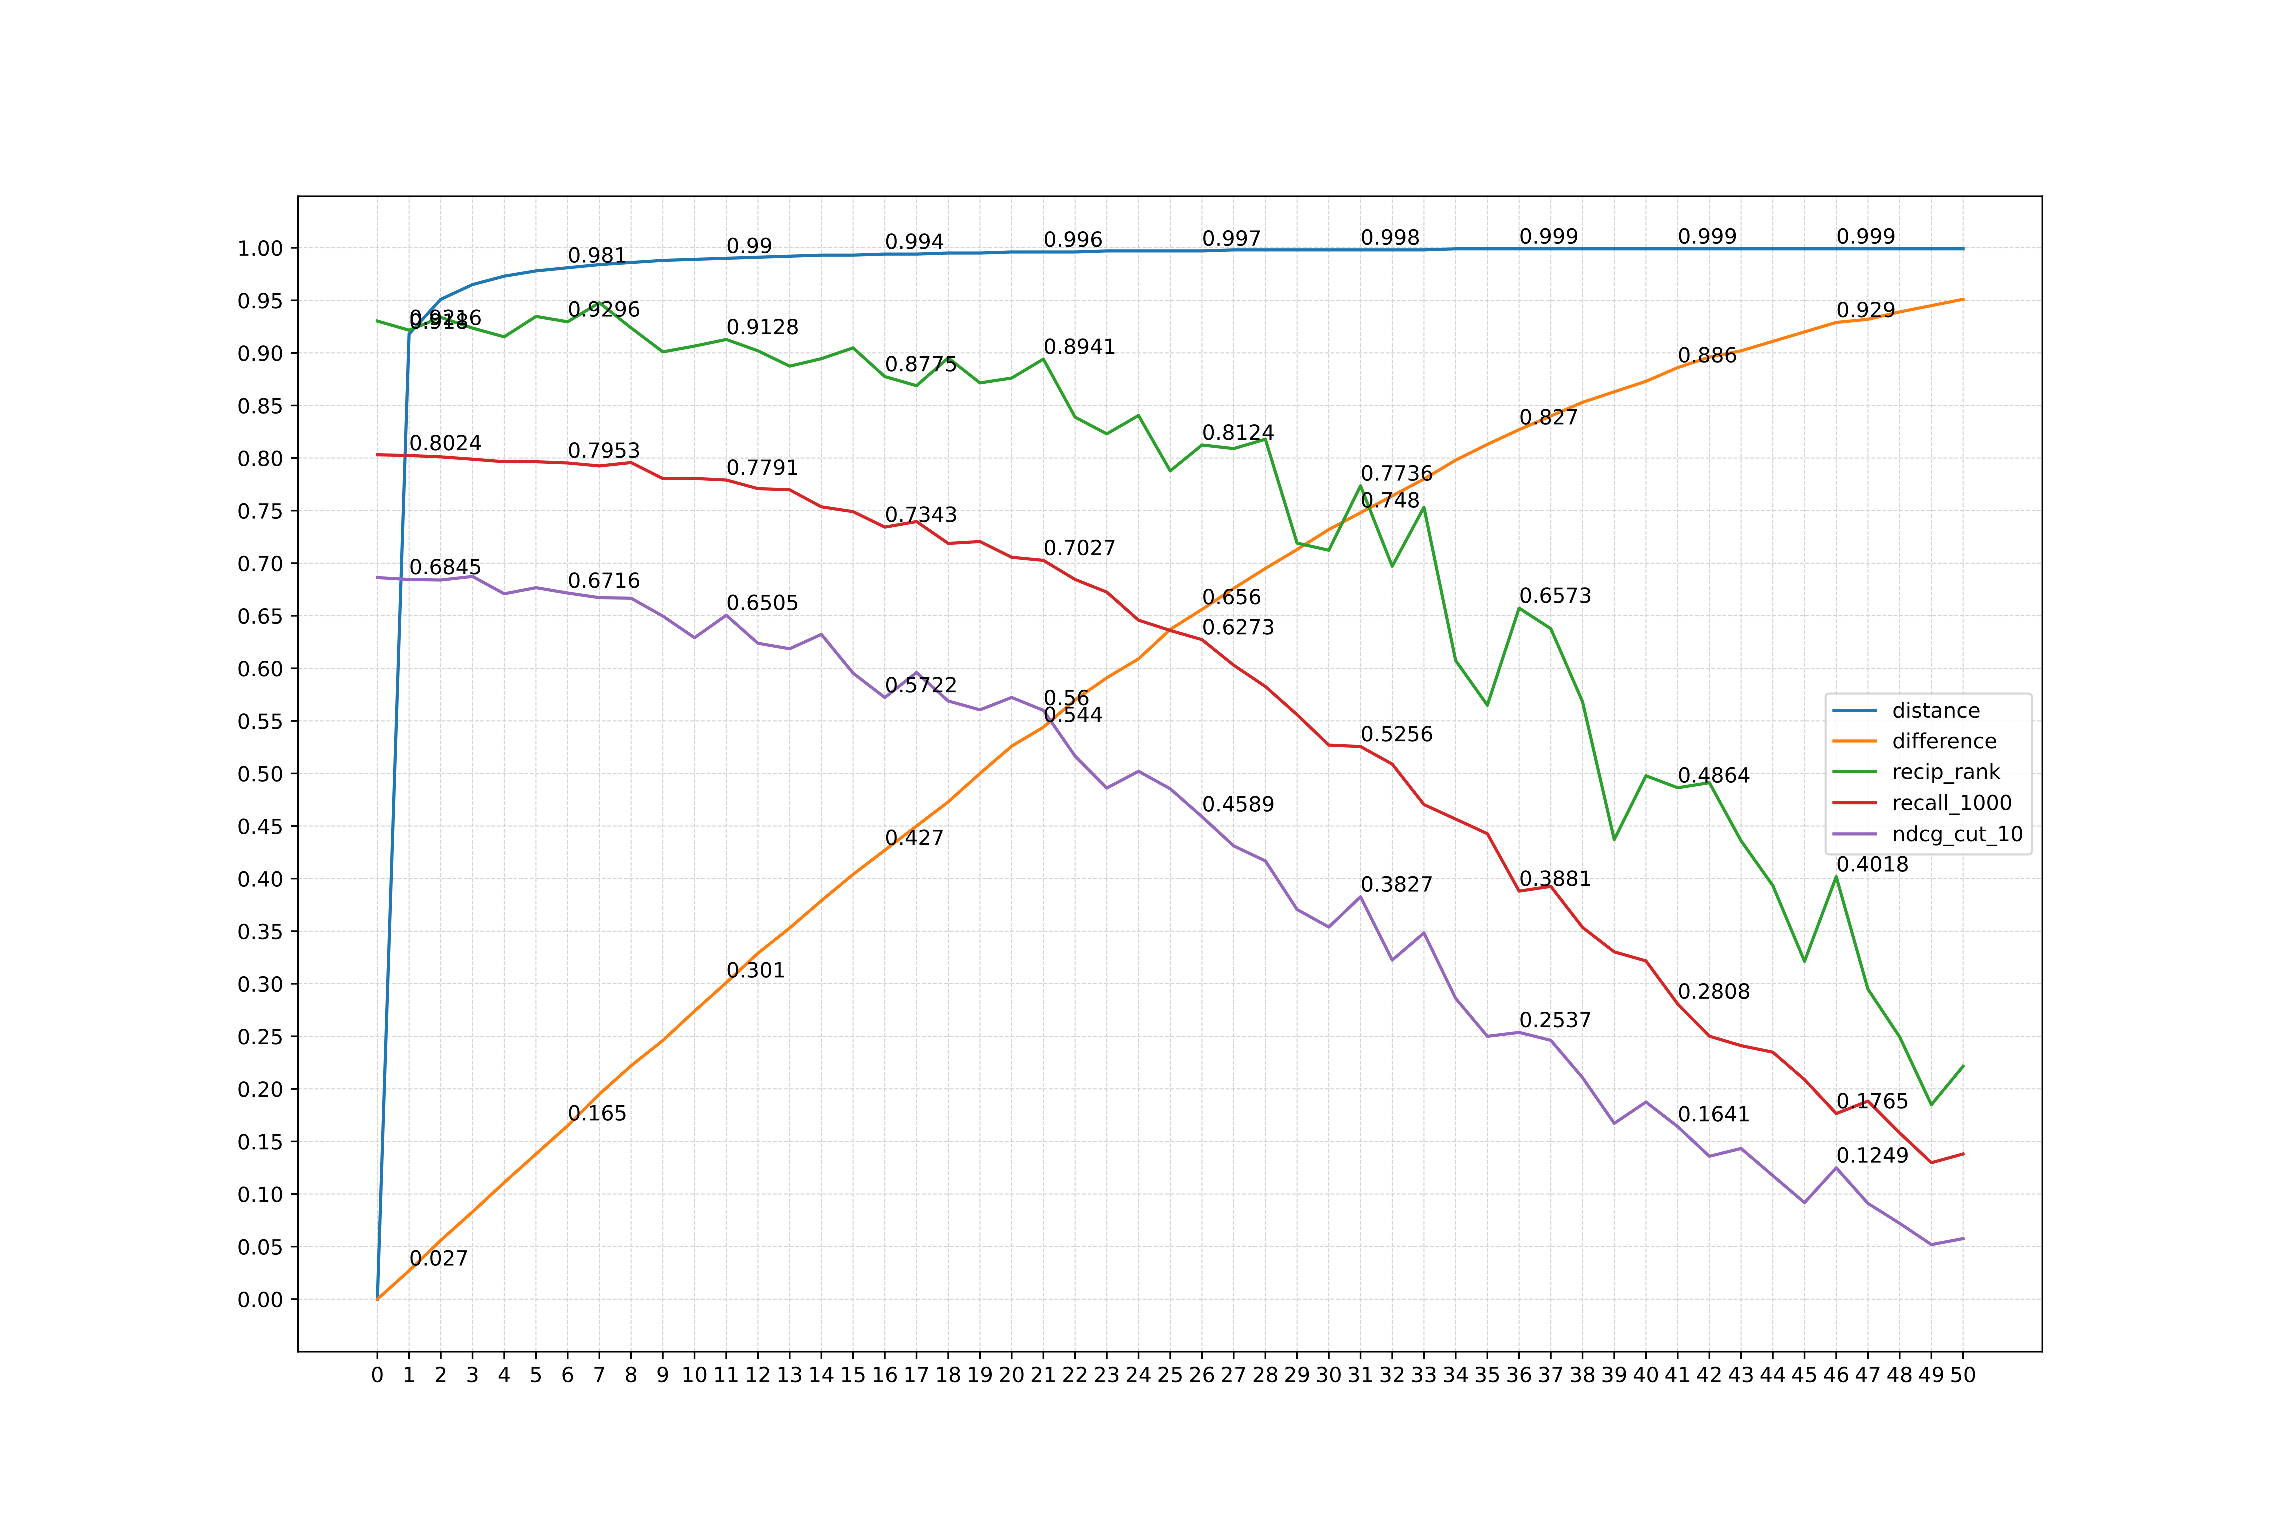
\includegraphics[trim=60 60 60 60,clip,width=0.75\textwidth]{knn}
			\caption{TREC metrics, result set distance and difference, for running \knn{} search for $\beta \in \{ 0, 1, \ldots , 50 \} $}
		\end{figure}

	\end{frame}
